%===================================
%===================================
%===================================
\setchapterpreamble[u]{\margintoc}
\chapter{Thermal desalination overview}
\labch{intro:desalination}

Desalination is increasingly recognized as a key strategy to address global 
freshwater scarcity, driven by the combined pressures of climate change and 
population growth. Regions already facing drought and water stress, such as 
parts of Spain, are expected to see growing dependence on desalinated water 
to meet rising demand. While desalination technologies—particularly 
membrane-based systems like Reverse Osmosis (RO)—have seen rapid expansion, 
the energy intensity of the process remains a major challenge. To mitigate 
this, efforts have focused on improving energy efficiency and integrating 
renewable energy sources such as solar or geothermal heat. In particular, 
thermal desalination technologies like Multi-Effect Distillation (MED) are 
gaining renewed interest due to their compatibility with low-exergy heat 
sources (e.g. waste heat) and the ability to treat high-salinity brines. These 
thermal processes also align better with circular economy approaches, allowing 
the concentration of brine and the recovery of valuable minerals such as 
lithium or magnesium, an emerging field known as brine mining.

%===================================
%===================================
\section{(Pendiente mover) Solar MED pilot plant description}
\labsec{intro:desalination:solarmed-pilot-plant}

The system is composed of three main components as shown in
\reffig{solarmed-pilot-plant-diagram}: a flat plate collector solar field which
is the heat source, a pressurized hot water two-tank thermal storage system,
and an MED plant which uses this heat to separate seawater into fresh water and
brine. The solar field and thermal storage circuits are separated by a heat
exchanger.

% TODO: A esta figura quitar colores de decision variable and environment
% variables, solo color neutro
\begin{figure*}[h!]
	\includegraphics[]{figures/SolarMED-process-diagram.png}
	\caption{SolarMED process diagram}
	\labfig{intro:desalination:solarmed-pilot-plant-diagram}
\end{figure*}


%===================================
%===================================
%===================================
\setchapterpreamble[u]{\margintoc}
\chapter{CSP overview}
\labch{intro:csp}

In the pursuit of eliminating reliance on fossil fuels sources for energy 
generation and replacing them by renewable sources, Concentrating Solar Power 
(CSP) has proven to be a reliable contributor. In particular, in providing much 
needed energy storage, dispatchability and ensuring grid stability.

% Introducción de artículo: Wet cooling tower performance prediction in CSP plants: A comparison between artificial neural networks and Poppe’s model
Concentrated Solar Power (CSP) plants use mirrors to concentrate the sun's
energy to finally drive a turbine that generates electricity. This technology
currently represents a minor part of renewable energy generation in Europe.
Only approximately 5~GW are installed globally (of which 2.3~GW in Europe are
concentrated in Spain). However, the potential for growth is significant given
the capability of CSP to provide renewable electricity when needed thanks to
in-built energy storage continuing the production even in the absence of
sunlight, unlike other renewable technologies that are dependent on the
availability of the energy source. Of increasing importance is also their
potential application in improving the manageability of the grid, replacing
fossil fuel alternatives. Their dispatchability enables plants to respond to
peaks in demand, and provide ancillary services to the grid. According to the
International Energy Agency forecasts, CSP has a huge potential in the long
term, ranging from the 986~TWh by 2030 up to 4186~TWh by 2050
\sidecite{iea_energy_2014}, which means that CSP will account for 11\% of the
electricity generated worldwide and for 4\% in the case of Europe. 

%================================
%================================
\section{Water use}
\labsec{intro:csp:water-use}

The cooling of the power block in this technology plays a crucial role in its
feasibility. The cheapest and most efficiency cooling technology is evaporative
cooling, and that is why most plants, specially in Spain where built using this
alternative (XX \% CSP data), however, the high-radiation areas in which they
are located are usually regions with rapidly-degrading water availability due
to climate change, so water has become a scarce resource. Nowadays most likely
those plants would have been built with dry cooling technologies, significantly
increasing the cost (up to 8\% during periods of high ambient temperatures when
energy demand and prices peak).

%===================================
%===================================
%===================================
\setchapterpreamble[u]{\margintoc}
\chapter{Cooling overview}
\labch{intro:cooling}

% Introducción de artículo: Wet cooling tower performance prediction in CSP plants: A comparison between artificial neural networks and Poppe’s model

Solar CSP plants are, in general, located in arid areas, where sun irradiance
is high but water is scarce. The efficiency of these plants is highly dependent
on the temperature at which the steam is condensed. To date, the conventional
systems used to remove excess heat from CSP plants are either wet
(water-cooled) or dry (air-cooled). The lowest attainable condensing
temperature is achieved in wet cooling systems that depend on the wet-bulb
temperature, allowing CSP plants to achieve higher efficiencies. However, this
efficiency increase is at the expense of a high cost: excessive water use. Dry
cooling systems eliminate the water use but they lead to lower plant
efficiencies when the ambient air temperature is high. Those hot periods are
often the periods of peak system demand and higher electricity sale price. The
combination of the advantages of each of them into an innovative cooling system
is thus of great interest. There are different types of innovative cooling
systems: those that integrate the dry and wet cooling systems into the same
cooling device, which are called hybrid cooling systems
\sidecite{rezaei_reducing_2010,asvapoositkul_comparative_2014,hu_thermodynamic_2018} 
and those that combine separate dry and wet cooling systems, which are called
combined cooling systems. In the case of hybrid cooling systems, the dry
section are composed of compact heat exchangers included in a wet cooling tower
\cite{rezaei_reducing_2010}. This kind of cooling systems can be considered
as an efficient cooling solution for CSP plants
\sidecite{elmarazgioui_impact_2022} due to the energy conservation and water
and greenhouse gas emissions savings. In the case of combined cooling systems,
different configurations can be found. The most commonly proposed in the
literature is the one that considers an Air Cooled Condenser (ACC) in parallel
with a Wet Cooling Tower (WCT), as can be seen in
\sidecite{barigozzi_wet_2011,barigozzi_performance_2014}. In this kind of
configuration, the exhaust steam from the turbine is condensed either through
the ACC or through a surface condenser coupled with the WCT. Another
configuration, recently proposed in \sidecite{palenzuela_experimental_2022} is
a wet and a dry cooling tower (type air cooled heat exchanger) sharing a
surface condenser. In this case, the exhaust steam from the turbine is
condensed through the surface condenser and the heated cooling water is cooled
either through the WCT or through the dry cooling tower. This kind of combined
cooling systems are proposed as the most suitable option for a flexible
operation as a function of the ambient conditions, since they allow to select
the best operation strategies to achieve an optimum water and electricity
consumption compromise \sidecite{asfand_thermodynamic_2020}. In addition, if
the optimization is combined with energy demand forecasting as described in
\sidecite{wazirali_stateoftheart_2023}, the expected results can be even
better.

%===================================
%===================================
\section{(Pendiente mover) Combined cooling pilot plant description}
\labsec{intro:cooling:cc-pilot-plant-description}

% TODO: Aquí habría que añadir una figura estilo diagrama de bloques, que no
% incluya solo el circuito de refrigeración, sino también los circuitos de
% intercambio y generación de calor.

The combined cooling pilot plant at the Plataforma Solar de Almería consists of
three circuits: cooling circuit (shown in Figure
\reffig{intro:cooling:cc-pilot-plant-diagram}), exchange circuit and heating
circuit. In the cooling circuit, water circulating inside the tube bundle of a
surface condenser is cooled through a wet cooling tower (WCT) and/or a dry
system (DC) of the air cooled heat exchanger (ACHE) type. Valves 1 and 2
(R$_p$, R$_s$, respectively) allow operation in different configurations: DC only, WCT only,
in series, in parallel with different opening percentages, or parallel-series.
In the exchange circuit, a saturated steam generator generates steam at
different pressures, which is in turn condensed through the Surface Condenser,
transferring its latent heat to the cooling water that is thus heated. Finally,
in the heating circuit, a static solar field provides the thermal energy
required by the steam generator using hot water as heat transfer fluid. A more
detailed description of this installation can be found in
\cite{palenzuela_experimental_2022}.

% TODO: A la salida de la segunda válvula hay que añadir una flecha para que
% sea más legible, renombrar válvulas V1 y V2 a Vp y Vs.
\begin{figure*}[h!]
	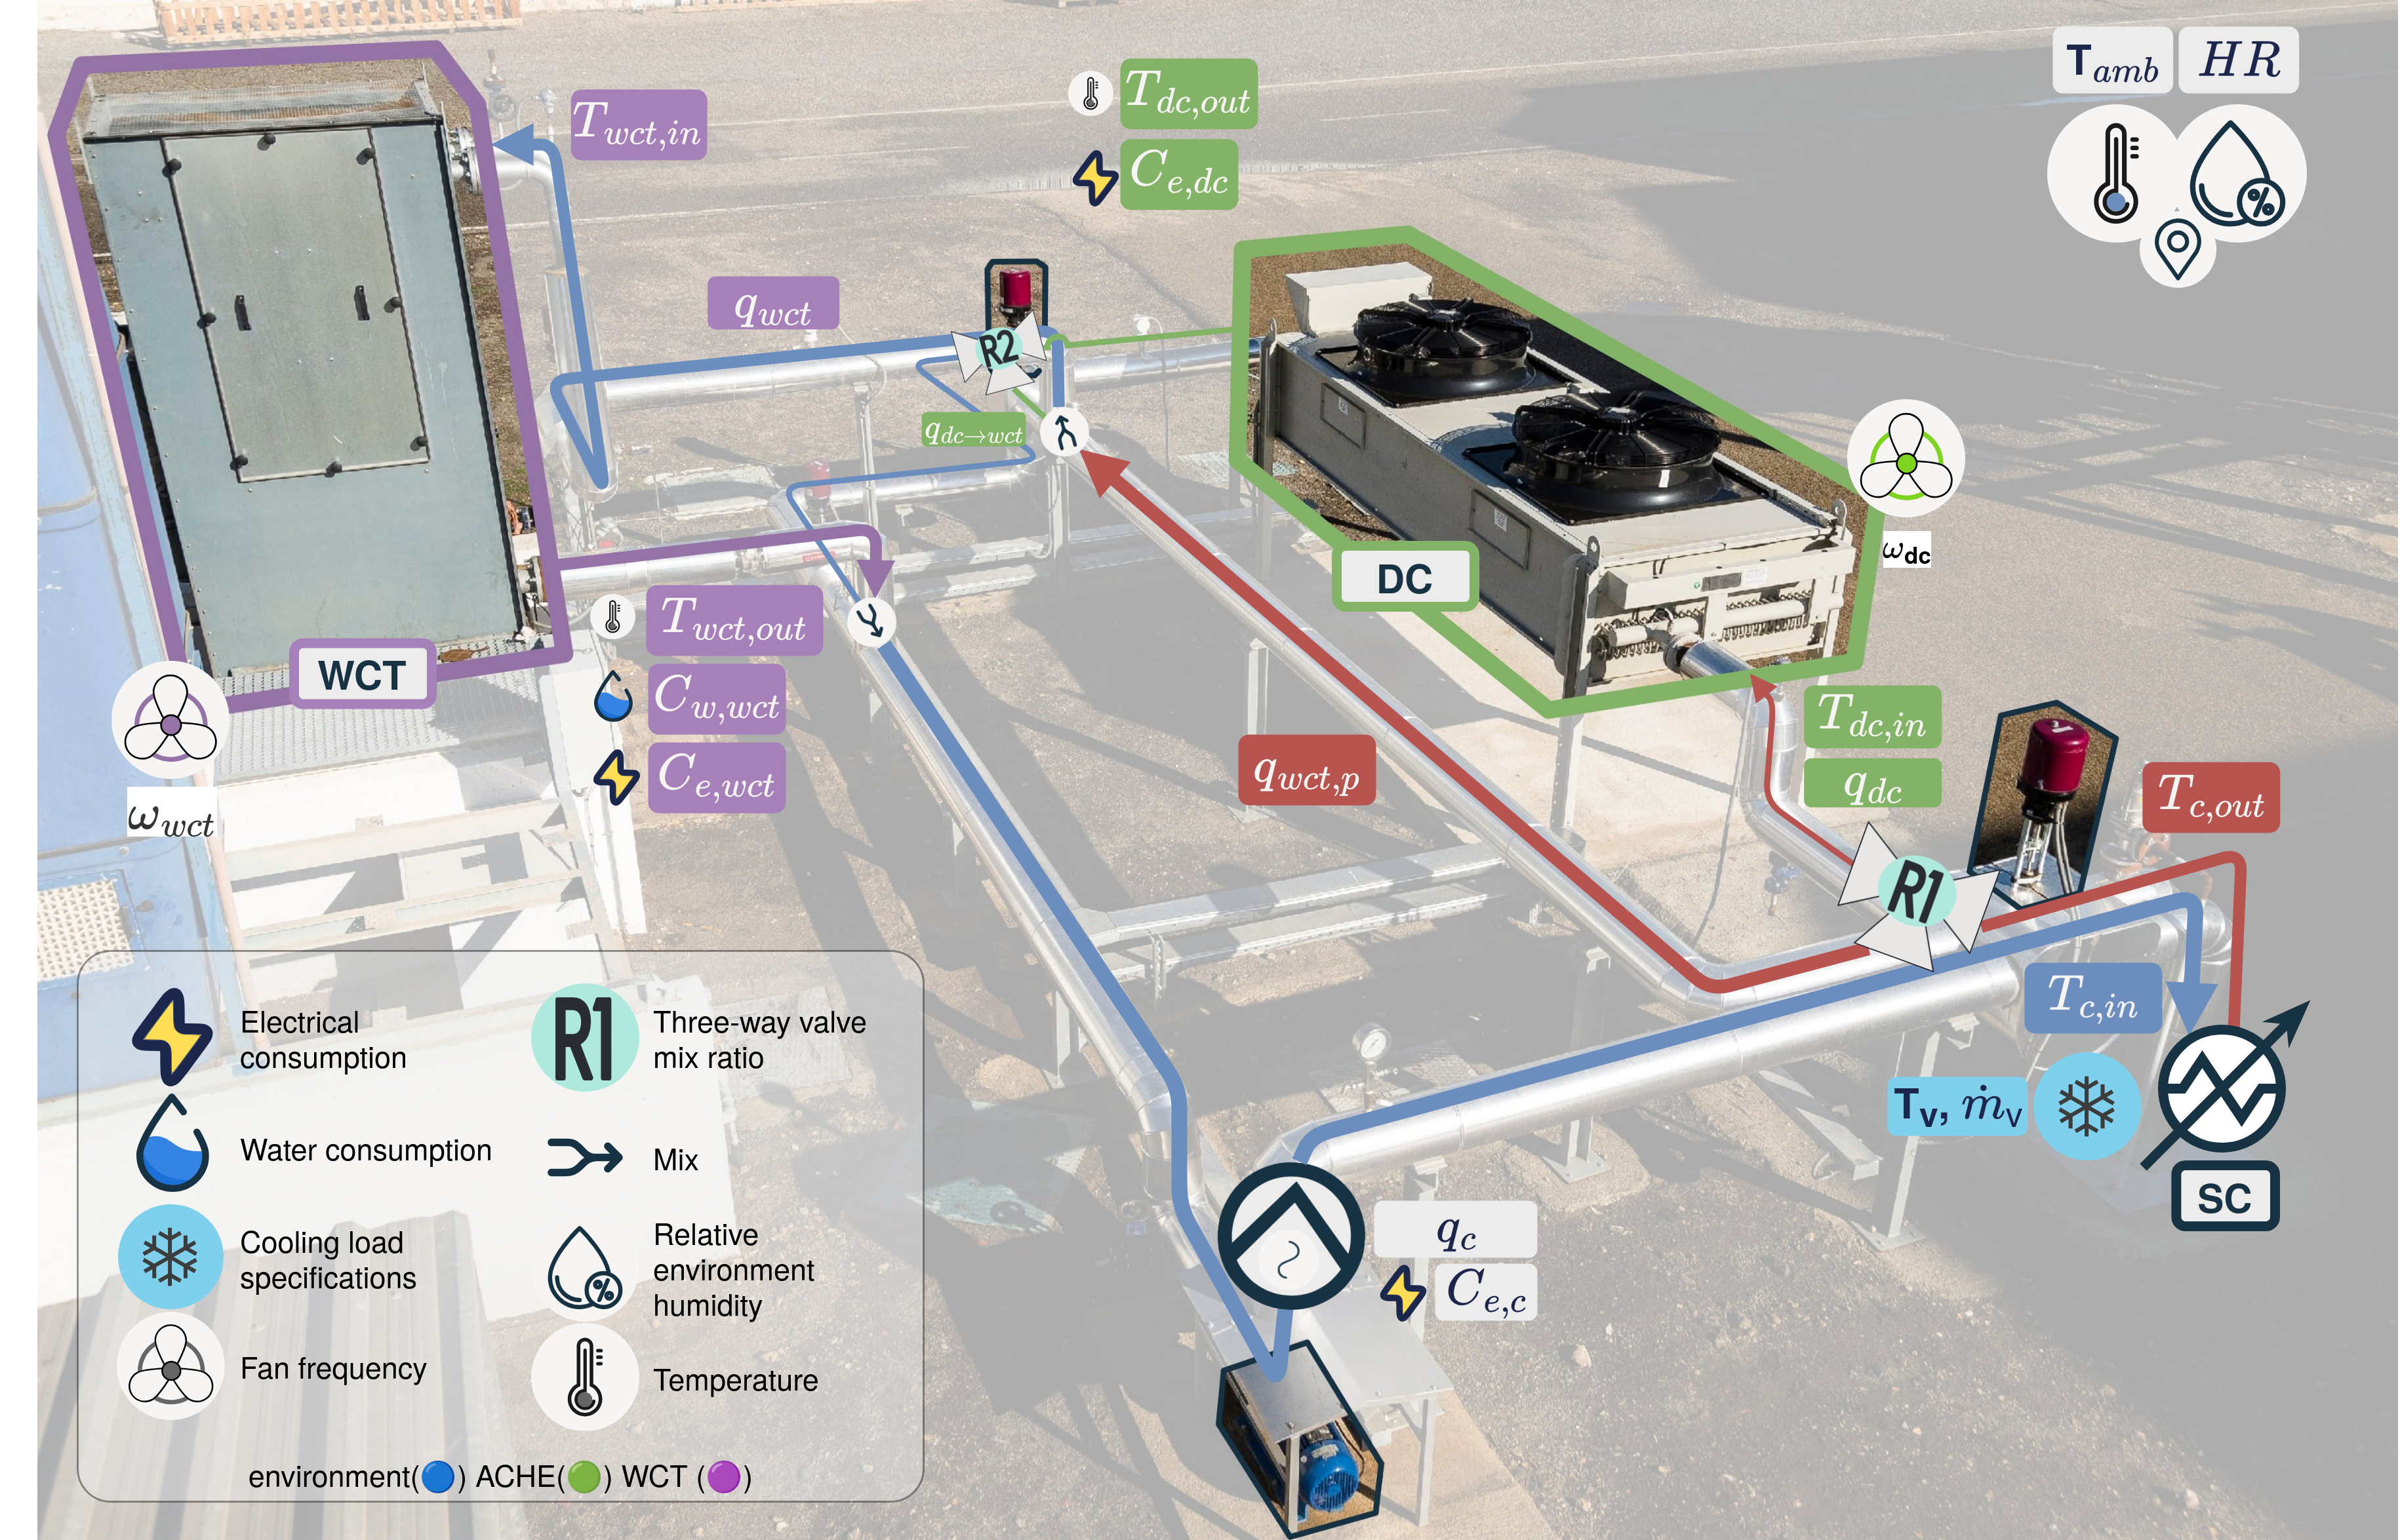
\includegraphics[]{figures/WASCOP-facility-diagram.png}
	\caption{PSA combined cooling system facility}
	\labfig{intro:cooling:cc-pilot-plant-diagram}
\end{figure*}

% Sacado de: Wet cooling tower performance prediction in CSP plants: A comparison between artificial neural networks and Poppe’s model
The pilot plant of combined cooling systems located at PSA  (see the layout in
\reffig{intro:cc:pilot-plant-pid}) consists of three circuits: cooling,
exchange and heating. In the cooling circuit (see a picture in
\reffig{intro:cc:pilot-plant-wct}), water circulating inside the tube bundle of
a Surface Condenser (SC) can be cooled through a Wet Cooling Tower and/or a Dry
Cooling Tower (type Air Cooled Heat Exchanger, ACHE), both with a designed
thermal power of 204~kW$_{th}$. In the exchange circuit, a saturated steam
generator of 80~kW$_{th}$ (on the design point), generates steam at different
pressures (in the range between 82~mbar and 200~mbar), which is in turn
condensed in the surface condenser. In this way, the steam transfers its latent
heat of condensation to the refrigeration water, that is heated. Finally, in
the heating circuit, a solar field with a thermal power of 300~kW$_{th}$ at the
design point, provides the energy required by the steam generator, in the form
of hot water. It is a unique, very flexible, fully instrumented and versatile
facility, able to operate in different operation modes: series and parallel
mode, conventional dry-only mode (all water flow is cooled through the dry
cooling tower) and wet-only mode (all water flow is cooled through the wet
cooling tower). The instrumentation related to the WCT is described in Table
\reftab{intro:cc:pilot-plant-instr}. Note that the sensors measuring the air
velocity and temperature and relative humidity at the outlet area of the wet
cooling tower have not been installed in the plant. Portable sensors were used
instead in some experiments, as described in Section \ref{sec:Data1}.

\begin{marginfigure}[-7cm]
    \includegraphics[]{figures/WASCOP-facility-WCT.png}
    % \caption{Back view of the WCT}
    \savebox\captionqr{\qrcode[hyperlink,height=0.4in]{\repositoryBaseUrl/figures/day_viz_20220614_eval_at_20250414T1247_test_water_price.html}}
	\caption[Back view of the WCT]{Back view of the WCT.\hspace{1ex}\usebox\captionqr}
    \labfig{intro:cc:pilot-plant-wct}
\end{marginfigure}

In regards to operational aspects of the the system, note that the cooling
water and air flow rates at the experimental facility ($\dot{m}_w$, and air,
$\dot{m}_a$, respectively), are modified with the \textit{Pump 1} and the fan
frequency percentage \texttt{SC-001}, respectively (see \reffig{intro:cc:pilot-plant-pid}). 


\begin{table}[h]
\caption{Characteristics of instrumentation ($^a$ value of the temperature in $^\circ$C, $^b$ of reading, $^c$ full scale, $^d$ mean value).} 
\labtab{intro:cc:pilot-plant-instr}
\resizebox{\linewidth}{!}{
\begin{tabular}{cccc} 
    \toprule
    \textbf{Measured variable} & \textbf{Instrument} & \textbf{Range}  & \textbf{Measurement uncertainty}\\
    \midrule
    Water temperature & Pt100 & 0 - 100 $^\circ$C & 0.03 + 0.005$\cdot T^a$\\
    (\texttt{TT-001}, \texttt{TT-006}) & & &\\
    Cooling water flow rate & Vortex flow meter & 9.8 - 25 m$^3$/h & $\pm$ 0.65 \% o.r.$^b$\\
    (\texttt{FT-001})  & & &\\
    Water flow rate  & Paddle wheel & 0.05 - 2 m$^3$/h & $\pm$ 0.5 \% of F.S$^c$  \\
    (\texttt{FT-004}) & flow meter  & & + 2.5 \% o.r\\
    Ambient temperature & Pt1000 & -40 - 60 $^\circ$C  & $\pm$ 0.4 $@$20 $^\circ$C \\
    Relative humidity & Capacitive sensor & 0 - 98\% & $\pm$ 3 \% o.r $@$20 $^\circ$C  \\
            Air velocity & Impeller anemometer & 0.1-15$~\mbox{m s$^{-1}$}$ & $\pm$ 0.1$~\mbox{m s$^{-1}$}$ + 1.5 \%  o.r \\
            Outlet air temperature & Pt100   & -20-70$^\circ$C & $\pm 0.5^\circ$C \\
            Outlet air humidity & Capacitive sensor   & 0-100\%& $\pm$ 2\% \\
    \bottomrule
\end{tabular}
}
\end{table}

\begin{figure}
    \includegraphics[width=1\textwidth]{figures/WASCOP-facility-PID.png}
    \caption{Layout of combined cooling systems pilot plant at PSA.}
    \labfig{intro:cc:pilot-plant-pid}
\end{figure}

%===================================
%===================================
%===================================
\setchapterpreamble[u]{\margintoc}
\chapter{Modelling overview}
\labch{intro:modelling}

%===================================
%===================================
\section{Performance metrics}
\labsec{intro:modelling:metrics}

To evaluate the quality of the models fit to the experimental data, four
performance metrics were evaluated: coefficient of determination (R$^2$), Root
Mean Square Error (RMSE), Mean Absolute Error (MAE) and Mean Absolute
Percentage Error (MAPE). These metrics are described below.


\textbf{Coefficient of determination}. R$^2$ measures the proportion of the
variance in the predicted variable that can be attributed to the independent
variable(s), in this case the considered system inputs. Values close to one
indicate a better prediction accuracy. It is calculated as follows:

\begin{equation*}
    R^2 = 1 - \frac{\sum\limits_{i=1}^n (y_i - \hat{y}_i)^2}{\sum\limits_{i=1}^n (y_i - \bar{y})^2},
\end{equation*}

where $y_i$ is the measured or observed value for the output variable, in the
$i-th$ observation, $\hat{y}_i$ is the estimated value of the same variable and
$n$ is the total number of observations. Finally, $\bar{y}$ is the mean value
of the experimental values.


\textbf{Root Mean Square Error}. RMSE is a statistical measure of the
difference between the values predicted by a model and the observed values. It
is calculated as the square root of the mean of the squared differences between
the predicted and observed values and it has its units. 

% \marginnote{
\begin{equation*}
    \mbox{RMSE} = \sqrt{\frac{1}{n} \sum\limits_{i=1}^n (y_i - \hat{y}_i)^2}
\end{equation*}
% }

\textbf{Mean Absolute Error}. It represents the average absolute difference
between predicted and actual values.

\begin{equation*}
    \mbox{MAE} = \frac{1}{n} \sum\limits_{i=1}^n \left|y_i - \hat{y}_i\right|
\end{equation*}

\textbf{Mean Absolute Percentage Error}. As the MAE, it calculates the
difference between the predicted and the actual values, but in this case it
does so in relative terms:

\begin{equation*}
    \mbox{MAPE} = \frac{1}{n} \sum\limits_{i=1}^n \left| \frac{y_i - \hat{y}_i}{y_i} \right| \times 100\%
\end{equation*}



%===================================
%===================================
\section{First principle modelling}
\labsec{intro:modelling:first-principle}

%===================================
%===================================
\section{Data-driven modelling}
\labsec{intro:modelling:data-driven}

Machine learning algorithms are unique in their ability to obtain models and
extract patterns from data, without being explicitly programmed to do so. They
are more effective with large volumes of data but can also be applied to build
steady state regression models with fewer information of a process.

%================================
\subsection{Gaussian Process Regression}
\labsec{intro:modelling:gpr}

%================================
\subsection{Artificial Neural networks}
\labsec{intro:modelling::ann}

Artificial neural networks (ANNs), as the name suggests, have a behavior
similar to biological neurons. Their structure is formed by a succession of
layers, each one composed by nodes (or neurons) and they receive as input the
output of the previous layer. This process is subsequently repeated until the
final layer which has a number of neurons equal to the number of outputs.

There are important aspects to be considered in the ANN model design, such as
the model configuration, the network architecture and the network topology.
They are discussed below.

% Configuraciones de modelo
\textbf{Model configuration}. The WCT model has two outputs, and thus several
configurations are available for the implementation of the model as shown in
 \ref{fig:model_configuration}. The first one is a  Multiple Inputs -
Multiple Outputs (MIMO) configuration, where a single network receives the five
defined inputs and directly produces the two desired outputs. The second one is
a cascade structure. This cascading approach involves training a network
(\textit{network A} in  \ref{fig:model_configuration} (b)) to predict the
outlet water temperature using the initial five inputs. Subsequently, these
inputs, along with the output from the temperature-predicting network, are fed
into a second network (\textit{network B} in  \ref{fig:model_configuration}
(b)) that is in charge of forecasting the system's water consumption. A
potential advantage of this configuration is that it may reduce the
experimental data requirements to obtain satisfactory results. 

% \begin{figure}%
%     \centering
%     \subfloat[\centering MIMO
%     configuration]{{\includegraphics[width=0.5\textwidth]{figures/ann_odel_configuration_mimo_with_legend.eps}
%     }}%
%     \qquad
%     \subfloat[\centering Cascade
%     configuration]{{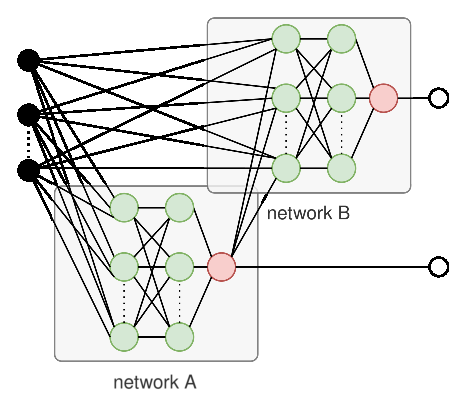
\includegraphics[width=0.4\textwidth]{figures/ann_model_configuration_cascade.eps}
%     }}%
    
%     \caption{ANN model configurations considered}%
%     \label{fig:model_configuration}%
% \end{figure}

%As a result, this approach holds the promise of enhanced efficiency in model
%training, potentially requiring fewer data points for accurate predictions. 

% Tipos de red Feedforward Cascade-forward Radial-basis
\textbf{Network architectures}. Three network architectures have been
implemented and tested:
\begin{enumerate}
    \item Feedforward network (FF) -  \ref{fig:ann_architectures} (a). This
    is the base network architecture, where different layers are added
    sequentially and the flow of information is unidirectional. The transfer
    function adopted in the hidden layers is the differentiable
    \textit{Log-Sigmoid}, whereas the one employed in the output layer is a
    linear one with no saturations.

    \item Cascade-forward network (CF) -  \ref{fig:ann_architectures} (b).
    It is a variation on the feedforward network since it adds direct
    connections from the input and hidden layers to the output layer.

    \item Radial-basis function network (RBF) - 
    \ref{fig:ann_architectures} (c). The transfer functions used in the first
    layer of the RBF network are different, they are local Gaussian like
    functions. Also, instead of multiplying by the weights, the distance
    between inputs and weights is computed and the bias is multiplied instead
    of added \sidecite{hagan_neural_2014}.
\end{enumerate}

% \begin{figure}%
%     \centering
%     \subfloat[\centering
%     Feedforward]{{\includegraphics[width=0.25\textwidth]{figures/neuron_type_simple_with_partial_legend.eps}
%     }}%
%     \qquad
%     \subfloat[\centering
%     Cascade-forward]{{\includegraphics[width=0.25\textwidth]{figures/neuron_type_cascade_with_partial_legend.eps}
%     }}%
%     \qquad
%     \subfloat[\centering
%     Radial-basis]{{\includegraphics[width=0.25\textwidth]{figures/neuron_type_radial_with_partial_legend.eps}
%     }}%
    
%     \caption{Considered ANN architectures.}%
%     \label{fig:ann_architectures}%
% \end{figure}

% topologías de red N de capas N de neuronas por capa

\textbf{Network topology}. Two-layer networks (one hidden and one output layer)
can learn almost any input-output relationship, including non-linear ones.
Adding more layers can improve the learning for more complex problems. However,
increasing the number of layers or neurons per layer increases the training
computational requirements, requires more data for a satisfactory model and can
lead to overfitting. Therefore, the process is usually started with two layers
and then the number of layers is increased if they do not perform
satisfactorily \sidecite{hagan_neural_2014}. In this study, for the feedforward and
cascade-forward architectures, one and two hidden layers have been tested with
the following configurations: 5, 10, 20, 5-5, 5-10, 10-5, 10-10. For the case
of the RBF, it only has one hidden layer and neurons are added sequentially
during the training process up to a maximum which is set to 120 neurons.

% Procedimiento entrenamiento Justificar mejor elección de algoritmo de
% entrenamiento
\textbf{Training process}. The next important aspect to consider is the
training process. For the FF and CF networks many Gradient- or Jacobian-based
algorithms can be utilized. In this case, the Levenberg-Marquardt
backpropagation algorithm \sidecite{beale2010neural} has been used. It is a fast
algorithm, ideal for multilayer networks with up to a few hundred weights and
biases enabling efficient training. The training in this case is done in
batches since sequential training is slower and does not produce better
results. All data have been normalized applying the z-score normalization
method. 
% Early stop, paciencia For most applications of neural networks, the training
% error never converges to exactly zero. The error can reach zero for the
% perceptron network (radial basis network), but it is unlikely to happen for
% multilayer networks. For this reason, a criteria for deciding when to stop
% the training needs to be set in place, and this criteria needs provide a
% mechanism to avoid overfitting. 
The criteria established for deciding when to stop the training is the
following one:  when the performance on the validation set increases (worsens)
or when the  gradient is below a minimum ($1\times10^{-7}$) for a number of
iterations or epochs, or when a maximum number of 1000 epochs is reached. The
number of iterations to wait, often refereed as patience, is set to 6. Finally,
the selected network parameters will be those of the best epoch.

For each network architecture, the training process was repeated a total of ten
times (this is the recommended practice if the computational requirements allow
it, since it guarantees reaching a global optimum with a high degree of
confidence \sidecite{hamm_comparison_2007}). The optimal architecture and training
was selected according to a performance function, which in this case has been
the Mean Square Error (MSE) with the values normalized.

In the case of the RBF network, the chosen training method consists in two
stages which treats the two layers of the RBF network separately. The first
layer weights and biases are tuned based on the orthogonal least squares method
\sidecite{hagan_neural_2014}, while for the second layer are computed in one step
using a linear least-squares algorithm. During training, neurons are added to
the first layer (in increments of 20) trying to minimize the MSE to some goal,
which in this case is set depending on the case study: 10 for the MIMO
configuration and 0 ($^\circ$C$^2$) and 20 (l$^2$/h$^2$) for temperature and
water lost networks, respectively, for the cascade configuration. Finally, a
parameter called spread is used to set the first layer biases. Larger values of
this parameter promote a smoother approximation of the training data (more
generalization), conversely, lower values provide a more exact fit to the
training data . Values from 0.1 to 30 have been tested for this parameter.


%================================
\subsection{Random Forest}
\labsec{intro:modelling::random-forest}

%================================
\subsection{Gradient Boosting}
\labsec{intro:modelling::gradient-boosting}


%===================================
%===================================
\section{Hybrid modelling}
\labsec{intro:modelling:hybrid}

%===================================
%===================================
\section[DD from FP. Sample generation]{Data-driven from first-principles models. Sample generation}
\labsec{intro:modelling:sample-generation}

% Mencionar modelos basados en datos a partir de modelos físicos. Describir combinatoria sin detallar la combinatoria particular seguida para el modelo del CC.

%===================================
%===================================
%===================================
\setchapterpreamble[u]{\margintoc}
\chapter{Sensitivity analysis}
\labch{intro:sensitivity}

It involves systematically assessing how variations in input parameters impact
the model's outputs. In this case, the Sobol method
\sidecite{nossent_sobolsensitivity_2011}, which is a variance-based approach, has
been used. This method decomposes the total variance of the model output into
contributions from individual input parameters and their interactions. By
quantifying the relative importance of each parameter, Sobol analysis
facilitates the identification of influential factors, enabling a more nuanced
understanding of complex systems characterized by numerous interacting
variables (five in this case). Sobol sensitivity analysis provides a
quantitative basis for assessing the consistency and validity of results when
different approaches to model a system are compared. ANNs models with similar
sensitivity analysis outcomes to those of the physical model,  are likely to
capture the essential features of the system, offering a means to verify their
credibility and ensuring that the proposed solutions align with the underlying
physical principles. Therefore, Sobol sensitivity analysis emerges as a
powerful tool not only for understanding the system input-outputs
relationships, but also as a way to validate and compare various modelling
approaches. The sensitivity analysis has been performed using \textit{SAlib},
an open source sensitivity analysis tool for the Python programming language
\sidecite{herman_salib_2017,iwanaga_toward_2022}.


\setchapterpreamble[u]{\margintoc}
\chapter{Control overview}
\labch{intro:control}

asdad

%===================================
%===================================
\section{PID controllers}
\labsec{intro:control:pid}

%===================================
%===================================
\section{Hierarchical control}
\labsec{intro:control:hierarchical}

%===================================
%===================================
%===================================
\setchapterpreamble[u]{\margintoc}
\chapter{Optimization overview}
\labch{intro:optimization}

asdad


%===================================
%===================================
\section{NLP problems}
\labsec{intro:optimization:nlp_problems}

%===================================
%===================================
\section{MINLP problems}
\labsec{intro:optimization:minlp_problems}

%===================================
%===================================
\section{Multi-objective optimization}
\labsec{intro:optimization:multi-objective}

%===================================
%===================================
\section{Optimization algorithms}
\labsec{intro:optimization:algorithms}


%===================================
%===================================
%===================================
\setchapterpreamble[u]{\margintoc}
\chapter{Research plan}
\labch{intro:plan}
% Fijarse en Tesis Simon

asdad

%===================================
%===================================
\section{Hypothesis}
\labsec{intro:research-plan:hypothesis}

%===================================
%===================================
\section{Objectives}
\labsec{intro:research-plan:objectives}


%===================================
%===================================
%===================================
\setchapterpreamble[u]{\margintoc}
\chapter{Contributions}
\labch{intro:contributions}

% Generales de la tesis, abstracto
asdad